\section*{Appendix}
\addcontentsline{toc}{section}{Appendix}

\subsection{Web-Based Platform for Data Partitioning Evaluation}\label{subsec:web_platform}

\begin{figure*}[h]
    \centering
    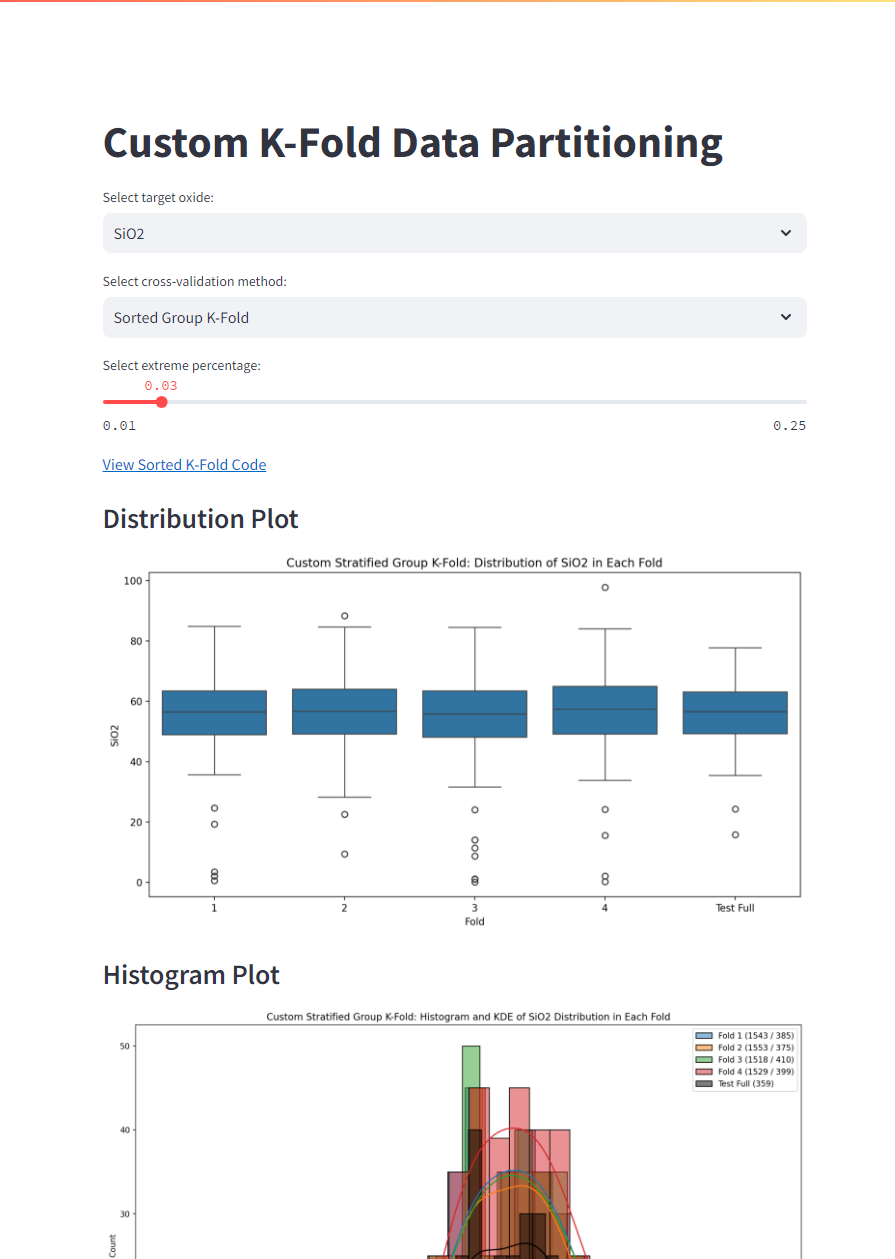
\includegraphics[width=\textwidth]{images/web_platform.png}
    \caption{Web-based platform used to determine the optimal value of $p$ for the data partitioning algorithm.}
    \label{fig:web_platform}
\end{figure*}

\subsection{Cross-Validation Plots for Major Oxides}\label{subsec:cv_plots}

% Loop through each major oxide and add a subsubsection with figures
\foreach \oxide in {SiO2, TiO2, Al2O3, FeOT, MgO, CaO, Na2O, K2O} {
    \subsubsection{\oxide}

    \begin{figure*}[h!]
        \centering
        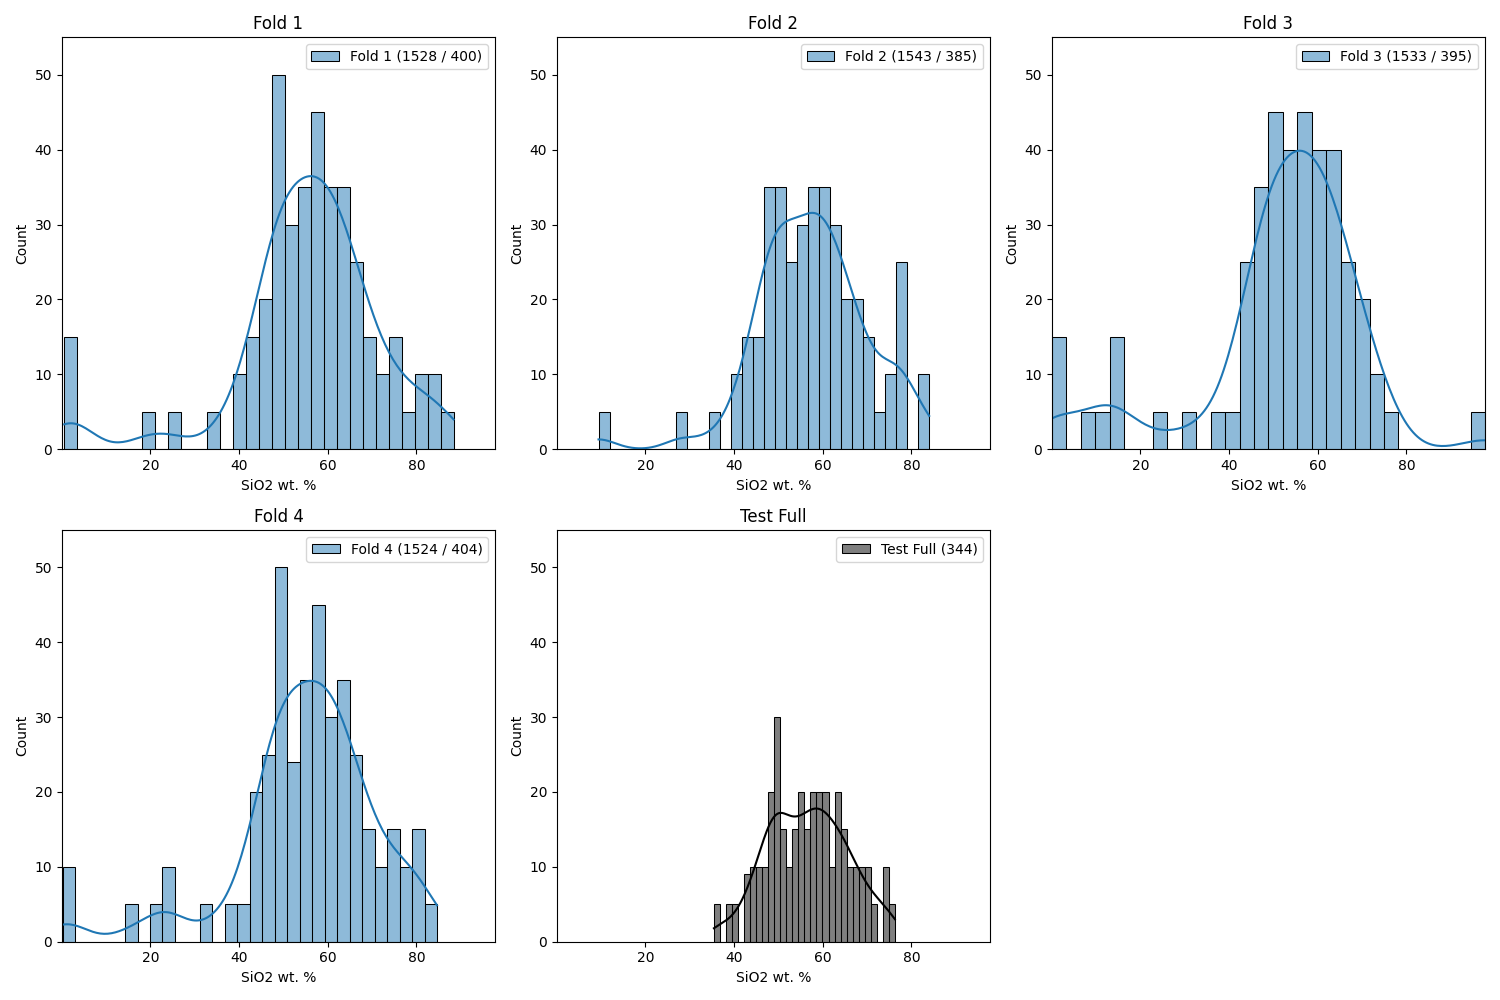
\includegraphics[width=\textwidth]{images/\oxide/histogram_grid_plot.png}
        \caption{Histogram and \gls{kde} of \ce{\oxide} distribution in each fold. The y-axis represents the count of samples per bin, and the x-axis represents \ce{\oxide} concentration. The notation in the legend indicates the amount of instances in the training/validation sets.}
        \label{fig:histogram_grid_plot_\oxide}
    \end{figure*}

    \begin{figure*}[h!]
        \centering
        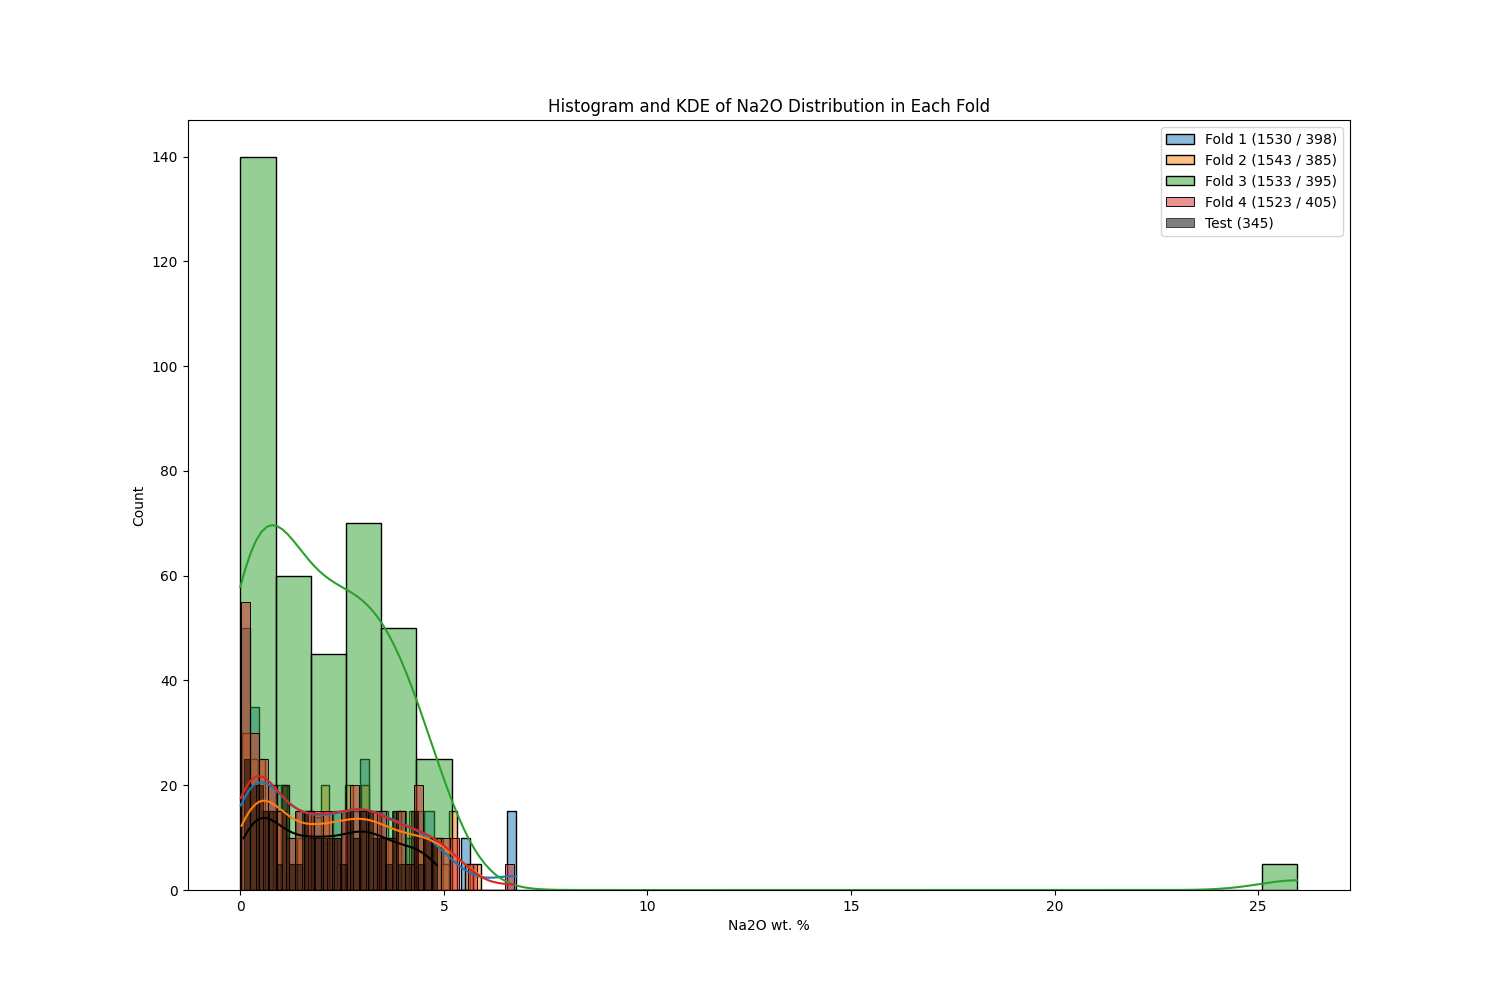
\includegraphics[width=\textwidth]{images/\oxide/histogram_kde_plot.png}
        \caption{Combined Histogram and \gls{kde} of \ce{\oxide} distribution in each fold. The y-axis represents the count of samples per bin, and the x-axis represents \ce{\oxide} concentration. The notation in the legend indicates the amount of instances in the training/validation sets.}
        \label{fig:histogram_kde_plot_\oxide}
    \end{figure*}

    \begin{figure*}[h!]
        \centering
        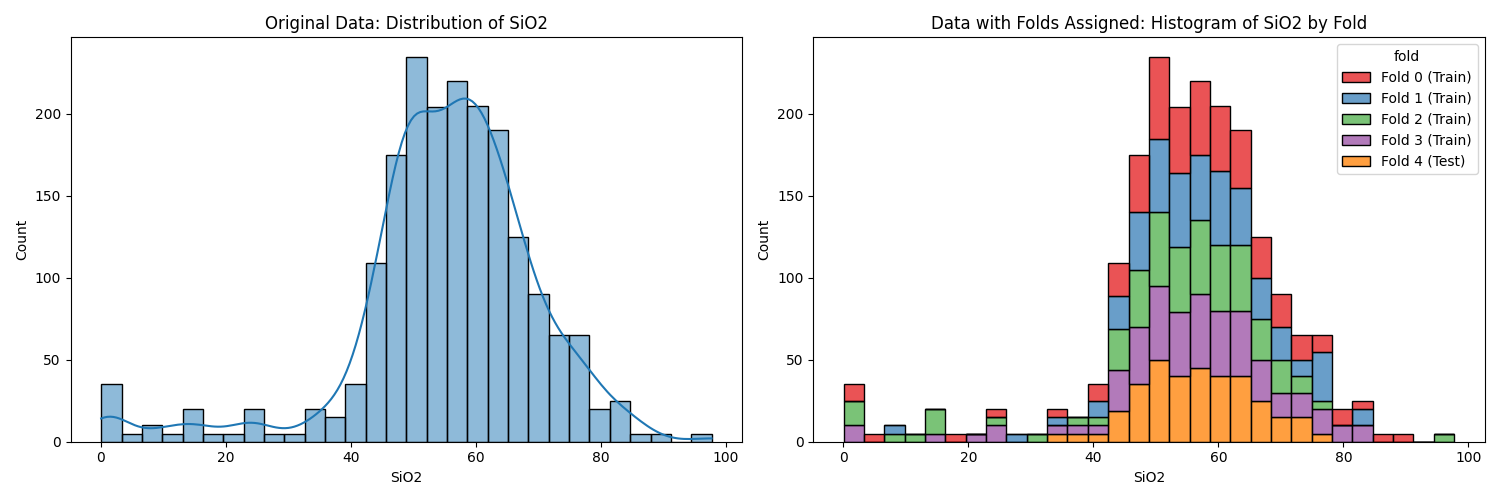
\includegraphics[width=\textwidth]{images/\oxide/original_and_post_fold.png}
        \caption{Distribution of \ce{\oxide} concentrations before and after fold assignment. The left plot shows the original distribution of \ce{\oxide}, while the right plot shows the distribution with folds assigned, color-coded to indicate the different folds.}
        \label{fig:original_and_post_fold_plot_\oxide}
    \end{figure*}

    \begin{figure*}[htbp]
        \centering
        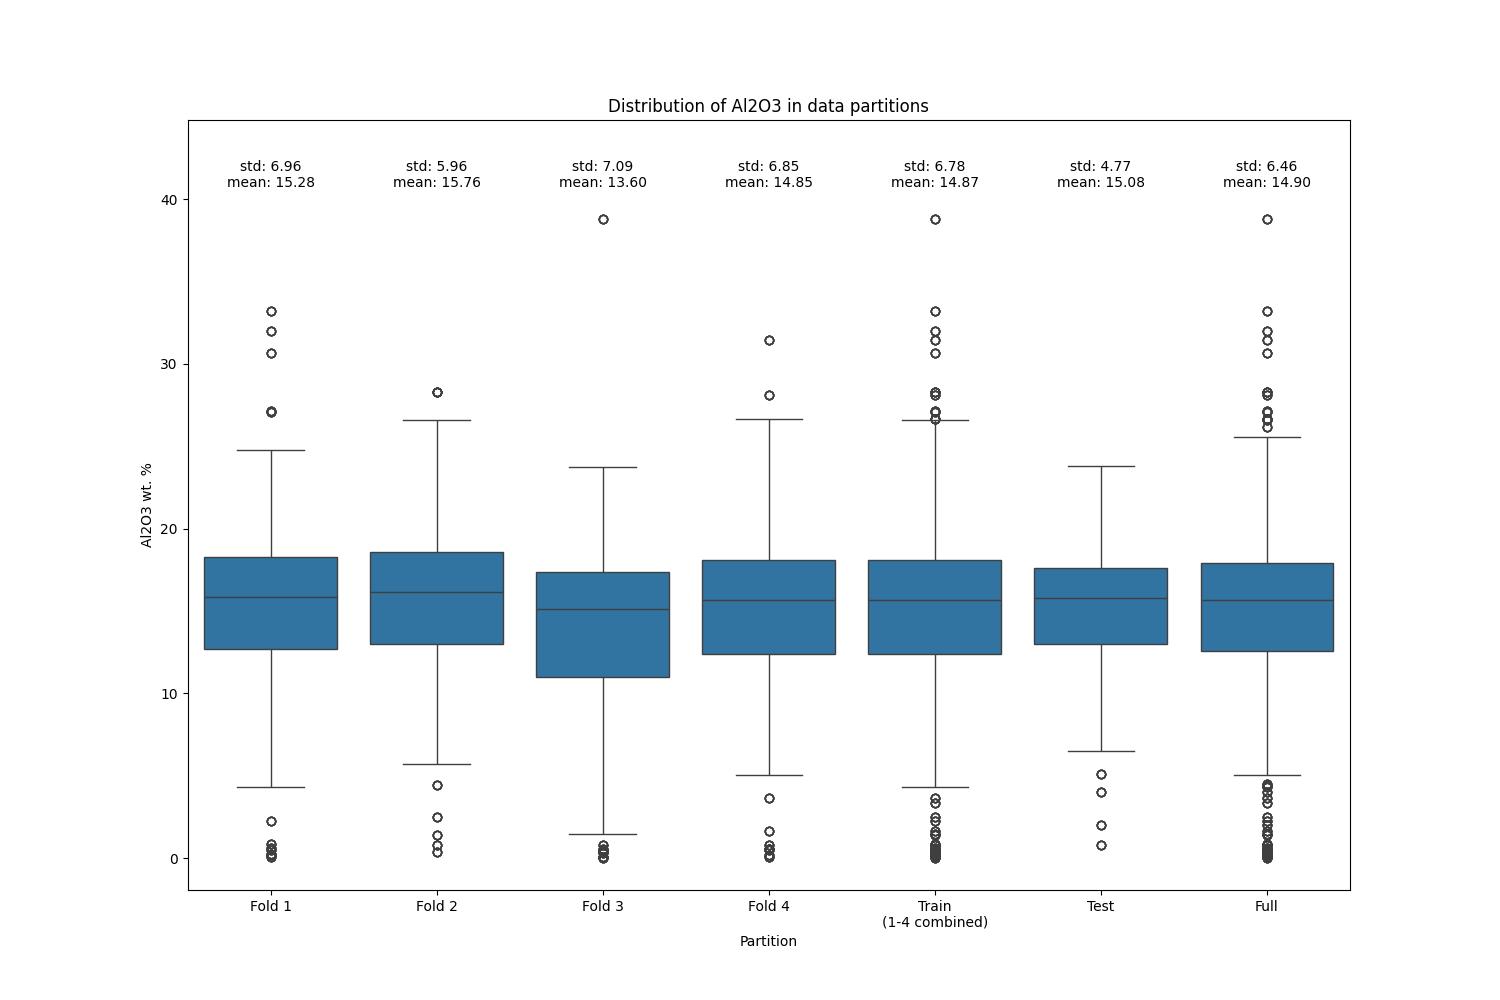
\includegraphics[width=\textwidth]{images/\oxide/distribution_plot.png}
        \caption{Distribution of \ce{\oxide} concentrations across cross-validation folds, training set, test set, and the entire dataset. The mean and standard deviation statistics for each partition are indicated figure.}
        \label{fig:distribution_plot_\oxide}
    \end{figure*}
}

\subsection{Initial Experiment: Model Hyperparameters}\label{subsec:initial_experiment_hyperparameters}
This section provides a detailed overview of the hyperparameters used for the models in the initial experiment.

\begin{table}[H]
\centering
\caption{Hyperparameters for Partial Least Squares}
\begin{tabular}{ll}
    \toprule
    \textbf{Hyperparameter} & \textbf{Value} \\
    \midrule
    Number of Components & 34 \\
    Scale & True \\
    Max Iter & 500 \\
    \bottomrule
\end{tabular}
\label{tab:pls_hyperparameters}
\end{table}
\FloatBarrier

\begin{table}[H]
\centering
\caption{Hyperparameters for Support Vector Regression}
\begin{tabular}{ll}
    \toprule
    \textbf{Hyperparameter} & \textbf{Value} \\
    \midrule
    Kernel & poly \\
    C & 100 \\
    Epsilon & 0.1 \\
    Gamma & scale \\
    Degree & 2 \\
    Coef0 & 1.0 \\
    \bottomrule
\end{tabular}
\label{tab:svr_hyperparameters}
\end{table}
\FloatBarrier

\begin{table}[H]
\centering
\caption{Hyperparameters for Elastic Nets}
\begin{tabular}{ll}
    \toprule
    \textbf{Hyperparameter} & \textbf{Value} \\
    \midrule
    Alphas & [0.0001, 0.001, 0.01, 0.1, 1, 10, 100, 1000] \\
    L1 Ratio & [0.1, 0.5, 0.7, 0.9, 1.0] \\
    Max Iter & 1000 \\
    Tolerance & 1e-4 \\
    \bottomrule
\end{tabular}
\label{tab:elasticnet_hyperparameters}
\end{table}
\FloatBarrier

\begin{table}[H]
\centering
\caption{Hyperparameters for Lasso}
\begin{tabular}{ll}
    \toprule
    \textbf{Hyperparameter} & \textbf{Value} \\
    \midrule
    Alphas & [0.0001, 0.001, 0.01, 0.1, 1, 10, 100, 1000] \\
    Max Iter & 1000 \\
    Tolerance & 1e-4 \\
    \bottomrule
\end{tabular}
\label{tab:lasso_hyperparameters}
\end{table}
\FloatBarrier

\begin{table}[H]
\centering
\caption{Hyperparameters for Ridge Regression}
\begin{tabular}{ll}
    \toprule
    \textbf{Hyperparameter} & \textbf{Value} \\
    \midrule
    Alphas & [0.0001, 0.001, 0.01, 0.1, 1, 10, 100, 1000] \\
    Max Iter & 1000 \\
    Tolerance & 1e-4 \\
    \bottomrule
\end{tabular}
\label{tab:ridge_hyperparameters}
\end{table}
\FloatBarrier

\begin{table}[H]
\centering
\caption{Hyperparameters for Random Forest}
\begin{tabular}{ll}
    \toprule
    \textbf{Hyperparameter} & \textbf{Value} \\
    \midrule
    Number of Estimators & 100 \\
    Max Depth & 10 \\
    Min Samples Split & 2 \\
    Min Samples Leaf & 1 \\
    Max Features & sqrt \\
    Random State & 42 \\
    \bottomrule
\end{tabular}
\label{tab:randomforest_hyperparameters}
\end{table}
\FloatBarrier

\begin{table}[H]
\centering
\caption{Hyperparameters for Gradient Boosting Regression}
\begin{tabular}{ll}
    \toprule
    \textbf{Hyperparameter} & \textbf{Value} \\
    \midrule
    Number of Estimators & 100 \\
    Max Depth & 3 \\
    Min Samples Split & 2 \\
    Min Samples Leaf & 1 \\
    Max Features & None \\
    Loss & squared\_error \\
    Learning Rate & 0.1 \\
    Subsample & 1.0 \\
    Criterion & friedman\_mse \\
    Random State & 42 \\
    Verbose & 0 \\
    Validation Fraction & 0.1 \\
    Number of Iterations No Change & None \\
    Tolerance & 1e-4 \\
    CCP Alpha & 0.0 \\
    \bottomrule
\end{tabular}
\label{tab:gbr_hyperparameters}
\end{table}
\FloatBarrier

\begin{table}[H]
\centering
\caption{Hyperparameters for Extra Trees Regression}
\begin{tabular}{ll}
    \toprule
    \textbf{Hyperparameter} & \textbf{Value} \\
    \midrule
    Number of Estimators & 100 \\
    Max Depth & 10 \\
    Min Samples Split & 2 \\
    Min Samples Leaf & 1 \\
    Random State & 42 \\
    \bottomrule
\end{tabular}
\label{tab:extratrees_hyperparameters}
\end{table}
\FloatBarrier

\begin{table}[H]
\centering
\caption{Hyperparameters for XGBoost}
\begin{tabular}{ll}
    \toprule
    \textbf{Hyperparameter} & \textbf{Value} \\
    \midrule
    Max Depth & 4 \\
    Min Child Weight & 5 \\
    Gamma & 0.1 \\
    Subsample & 0.7 \\
    Colsample Bytree & 0.5 \\
    Colsample Bylevel & 0.5 \\
    Colsample Bynode & 0.5 \\
    Lambda & 1 \\
    Alpha & 0.5 \\
    Learning Rate & 0.05 \\
    Number of Estimators & 100 \\
    Objective & reg:squarederror \\
    Eval Metric & rmse \\
    \bottomrule
\end{tabular}
\label{tab:xgboost_hyperparameters}
\end{table}
\FloatBarrier

\begin{table}[H]
\centering
\caption{Hyperparameters for NGBoost}
\begin{tabular}{ll}
    \toprule
    \textbf{Hyperparameter} & \textbf{Value} \\
    \midrule
    n/a & n/a \\
    \bottomrule
\end{tabular}
\label{tab:ngboost_hyperparameters}
\end{table}
\FloatBarrier

\begin{table}[H]
\centering
\caption{Hyperparameters for Artificial Neural Networks}
\begin{tabular}{ll}
    \toprule
    \textbf{Hyperparameter} & \textbf{Value} \\
    \midrule
    Layer 1: Dense & (1024 units) \\
    Layer 2: Dropout & (rate: 0.5) \\
    Layer 3: Dense & (512 units) \\
    Layer 4: Dropout & (rate: 0.5) \\
    Layer 5: Dense & (256 units) \\
    Layer 6: Dense & (128 units) \\
    Layer 7: Dense & (1 unit) \\
    \bottomrule
\end{tabular}
\label{tab:ann_hyperparameters}
\end{table}
\FloatBarrier

\clearpage
\begin{table}[H]
\centering
\caption{Hyperparameters for Convolutional Neural Networks}
\begin{tabular}{ll}
    \toprule
    \textbf{Hyperparameter} & \textbf{Value} \\
    \midrule
    Layer 1: InputLayer & (6144, 1) \\
    Layer 2: BatchNormalization & (axis: -1) \\
    Layer 3: Conv1D & (filters: 64, kernel size: 3, activation: relu) \\
    Layer 4: MaxPooling1D & (pool size: 2) \\
    Layer 5: Conv1D & (filters: 64, kernel size: 3, activation: relu) \\
    Layer 6: MaxPooling1D & (pool size: 2) \\
    Layer 7: Conv1D & (filters: 64, kernel size: 3, activation: relu) \\
    Layer 8: Add & (merge with layer 6 output) \\
    Layer 9: Conv1D & (filters: 128, kernel size: 3, activation: relu) \\
    Layer 10: MaxPooling1D & (pool size: 2) \\
    Layer 11: Conv1D & (filters: 128, kernel size: 3, activation: relu) \\
    Layer 12: MaxPooling1D & (pool size: 2) \\
    Layer 13: Conv1D & (filters: 128, kernel size: 3, activation: relu) \\
    Layer 14: Add & (merge with layer 12 output) \\
    Layer 15: Flatten & (output) \\
    Layer 16: Dropout & (rate: 0.5) \\
    Layer 17: Dense & (512 units, activation: relu) \\
    Layer 18: Dense & (1 unit, activation: linear) \\
    \bottomrule
\end{tabular}
\label{tab:cnn_hyperparameters}
\end{table}
\FloatBarrier